\documentclass[a4paper,twocolumn,11pt,unpublished]{quantumarticle}
\pdfoutput=1
\usepackage[utf8]{inputenc}
\usepackage[english]{babel}
\usepackage[T1]{fontenc}
\usepackage{amsmath}
\usepackage{textcomp}
\usepackage{hyperref}
\usepackage{braket}
\usepackage[table]{xcolor}

\usepackage{graphicx}
\usepackage[textheight=20 cm, textwidth=15cm, headheight=50pt, headsep=10pt,
footskip=32pt]{geometry}
\usepackage{amsfonts}
\usepackage{todonotes}
\usepackage{qcircuit}
\usepackage{physics}
\usepackage{bm}
\usepackage{amssymb}
\usepackage{algorithm}
\usepackage{algpseudocode}

\usepackage{tikz}
\usepackage{lipsum}
% \usepackage{etoolbox}

% \usepackage[backend=biber]{biblatex}
% \addbibresource{qkd.bib}

\newcommand{\Id}{{\rm 1\hspace{-0.9mm}l}}
\newcommand{\C}{\ensuremath{\mathbb{C}}}
\newcommand{\PP}{\ensuremath{\mathcal{P}}}
\newcommand{\QQ}{\ensuremath{\mathcal{Q}}}
\newcommand{\R}{\ensuremath{\mathbb{R}}}
\renewcommand{\AA}{\ensuremath{\mathcal{A}}}
\newcommand{\BB}{\ensuremath{\mathcal{B}}}
\newcommand{\p}{\ensuremath{p_{\mathrm{I}}}}
\newcommand{\pp}{\ensuremath{p_{\mathrm{II}}}}
\newcommand{\proj}[1]{\ensuremath{\ketbra{#1}{#1}}}

\begin{document}
\title{Quantum Key Distribution With Single-Qubit Transmission}

\author{Ryszard Kukulski}
\email{ryszard.stefan.kukulski@vsb.cz}
\affiliation{IT4Innovations, VSB~-~Technical University of Ostrava,
17.~listopadu 2172/15, 708 33 Ostrava, Czech Republic}
\orcid{0000-0002-9171-1734}
\author{Paulina Lewandowska}
\affiliation{IT4Innovations, VSB~-~Technical University of Ostrava,
17.~listopadu 2172/15, 708 33 Ostrava, Czech Republic}
\orcid{0000-0003-1564-7782}
\maketitle

\begin{abstract}
The security of quantum key distribution (QKD) protocols is based on its
resilience to the existence of quantum errors created by the environment or the
eavesdropper.
In this work, we introduce a new QKD protocol that was specifically designed
to tolerate high levels of QBER (quantum bit error rate) and simultaneously
maintain reasonable security.
The protocol was tested and compared with other QKD protocols using
semidefinite programming (SDP). For this type of optimization, we use an
arbitrary decision function that can be seen as a generalization of the
post-selection scheme, used during classical communication to accept or reject
the measured outcome.
\end{abstract}

\section{Introduction}
Quantum cryptography studies cryptographic primitives whose security stems from
physical laws rather than computational assumptions. Beyond key agreement, the
area spans randomness generation, quantum money, secure delegated computation,
and multi-party cryptography; nonetheless, quantum key distribution (QKD)
remains the most mature primitive, with security reductions and implementations
across fiber, free-space, and networked settings
\cite{ScaraniRMP2009,PirandolaAOP2020}. Practical analyses close the gap between
idealized models and devices, detailing countermeasures against side channels
and implementation flaws \cite{XuRMP2020}. Architecturally, advances such as
measurement-device-independent QKD (MDI-QKD) mitigate detector attacks by
relocating measurements to an untrusted relay, while device-independent QKD
(DI-QKD) pushes toward security from observed nonlocal correlations alone
\cite{LoCurtyQi2012,DIQKDReview2023}. On the proof side, modern techniques
leverage symmetry reductions and post-selection/de Finetti methods to convert
observed statistics into finite-size key bounds compatible with realistic
experiments \cite{ChristandlRenner2009,ShorPreskill2000}.

This work takes a complementary route: we design a prepare-and-measure protocol
that explicitly exploits discrimination of quantum measurements. In particular,
we use results on single-shot discrimination of von Neumann measurements,
quantified via the diamond-norm distance and solvable by cone/semidefinite
programs, to inform our choice of preparation ensemble, Bob’s measurement
family, and a deterministic acceptance (post-selection)
rule~\cite{Puchala2018VNM}. Intuitively, acceptance regions that are hard for an
eavesdropper’s effective measurement to emulate, yet remain reliable for Bob,
enlarge the security margin at fixed quantum bit error rate (QBER). We formalize
the resulting Eve–Bob trade-off as an SDP, compare against BB84/MDI-style
sifting, and identify operating points where the induced
measurement-discrimination gap yields improved tolerable QBER without collapsing
the protocol’s success probability \cite{BB84,LoCurtyQi2012,Puchala2018VNM}.

Finally, we situate the protocol within the standard post-processing
pipeline—parameter estimation, error correction, and privacy
amplification—highlighting how the measurement-discrimination perspective
guides acceptance thresholds and finite-size budgeting
\cite{ScaraniRMP2009,XuRMP2020}.

\section{Protocol Landscape and Related Work}
Current QKD implementations span four practical classes: prepare-and-measure
protocols, entanglement-based protocols, measurement-device-independent (MDI)
protocols, and device-independent (DI) protocols
\cite{lo2014secure,XuRMP2020,LoCurtyQi2012,DIQKDReview2023}. BB84 and B92 remain
canonical prepare-and-measure references \cite{BB84,B92}, while six-state (SSP)
and SARG04 represent security-oriented variants that trade efficiency for
stronger disturbance sensitivity \cite{SSP,SARG04}. Entanglement-based baselines
such as E91 and BBM92 provide a different security viewpoint based on nonlocal
correlations and shared-state verification \cite{ekert1991quantum,B92ent}.

For high-rate or long-distance deployments, modern systems increasingly combine
implementation-layer improvements with protocol-level asymmetry. Representative
examples include unbalanced/decoy-inspired BB84 variants such as T12, and
twin-field style approaches that improve rate-distance scaling without trusted
repeaters \cite{T12,rate_distance}. Our protocol is positioned as a
prepare-and-measure design that explicitly optimizes the Bob-versus-Eve
discrimination gap under a single-qubit transmission model, rather than as an
MDI or DI construction.

\section{Results} 


We consider a basic QKD scheme involving two trusted parties, Alice and Bob, and
an adversary, Eve.  Eve's goal is to intercept or interrupt the exchange. There
exists a classical authenticated public channel, and the quantum channel which
is potentially private but remains susceptible to eavesdropping. Communication
is restricted to single qubit transmissions. 

Although the quality of the quantum channel increases over time, it can never be
flawless. Security analyses must therefore account for the presence of an
adversary (Eve). If the protocol is weak, Eve may extract information about the
key while remaining undetected, whereas a strong protocol presents an
opportunity to attempt a denial-of-service (DoS) attack by aborting
communication.

\subsection{Framework of the protocol} 
The general prepare and measure QKD-1q setup is presented in Fig.
\ref{fig-protocol}.
Alice sends a quantum state $\ket{\psi_a} \in \mathbb{C}^d$, 
randomly chosen according to a probability distribution $p_a$, 
with $a \in R_a = \{1, \ldots, |R_a|\}$. 
Bob performs a positive operator-valued measurement (POVM).
$\Omega = \{\proj{\phi_b}\}_b$ for $b \in R_b = \{1, \ldots, |R_b|\}$, obtaining
the outcome $b$. 
The operator $E$ describes a potential Eve attack.

\begin{figure}[htp!]
	\centering
    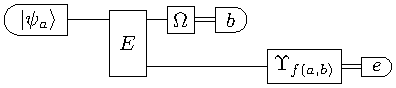
\includegraphics[width=1\linewidth]{figures/fig-protocol.pdf}
    \caption{The general setup of proposed framework}
    \label{fig-protocol}
\end{figure}

In the postprocessing stage, Alice and Bob communicate classically to reconcile
their outcomes. The goal of this step is to implement a deterministic decision
function $f(a,b)$ that maps the results of their measurements into a successful
key bit or an abort. Communication proceeds as an exchange of messages.
Eventually, the procedure stops, and an equivalence class of indexes (that
create the same sequence of messages) is obtained.
\begin{equation}
   f(a,b) = R_a(a,b) \times R_b(a,b) \ni (a,b).
\end{equation}
where $R_a(a,b) \subseteq R_a$ and $R_b(a,b) \subseteq R_b$. 

Each $f(a,b)$ determines whether the protocol is successful $S$ or failed. If
$S$, then Alice and Bob generate the key. For Alice, the key is $A=i$ if $a \in
R_a(a,b)_i$ for $i=0,1$, where $R_a(a,b)_0 \cup R_a(a,b)_1 = R_a(a,b)$ (for Bob
it is $B=i$ if $b \in R_b(a,b)_i$ with $R_b(a,b)_0 \cup R_b(a,b)_1 = R_b(a,b)$).

If $S$, then Eve try to determine the key value by implementing binary
measurement $\Upsilon_{f(a,b)}$. The Eve key is $e$.

\subsection{QKD-1q as a Black-Box}

The above framework allows us to treat concrete protocols (e.g., BB84,
six-state) as particular instances, while keeping the discussion independent of
implementation details.

To evaluate any such protocol within this framework, we introduce a set of
black-box measures expressed as probabilities.
\begin{itemize}
    \item Probability that the protocol will succeed $P(S)>0$.
    \item Probability of successful key generation $P(B=A|S)=1$.
    \item Probability of eavesdropping $P_E(E=A|S)$.
    \item Security check $P_E(b,a) \sim P(b,a)$.
\end{itemize}
These measures provide a unified way to assess the trade-offs between
reliability, key rate, and security. For example, a scheme can be constructed
such that $P(S) \to 1$ and $P(B=A \mid S)=1$, which maximizes the key generation
rate. However, in this limit, guaranteeing security requires
nearly perfect quantum channels, since even a small interaction with Eve can
lead to $P_E(S) \to 0$.

The use of the decision function $f(a,b)$ ensures that after postprocessing, the
protocol satisfies condition $P(A=B|S)=1$, i.e., whenever the protocol accepts,
the keys match perfectly.


\subsection{KL3P2W}
The protocol introduced below \ref{fig-qkd1q} is an implementation of the above
framework that tolerates moderate noise while still maintaining a high level of
security. Both Alice and Bob systems are two-dimensional Hilbert spaces,
\[
\mathcal{H}_A = \mathcal{H}_B = \mathbb{C}^2.
\]
\begin{figure}[htp!]
	\centering
    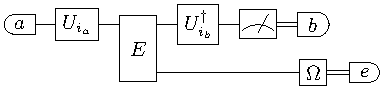
\includegraphics[width=1\linewidth]{figures/KL3P2W.pdf}
    \caption{The setup of KL3P2W protocol.}
    \label{fig-qkd1q}
\end{figure}
Alice prepares state $\ket{\psi_{r_a}}$, where $\psi_{r_a}=0$ with probability
$20\%$ and $\psi_{r_a}=1$ with probability $80\%$. Next, she applies a unitary
operator $U_{a_i}$, where $a_i \in \{1,2,3,4\}$ and sends the resulting qubit to
Bob. Bob performs a measurement on one of the four bases defined by a unitary
$U_{i_b}^\dagger$, where $i_b = \{1,2,3,4\} $. As a result, he obtains an
outcome $b \in \{0,1\}$.
 The protocol is successful if $b=0$, for $b=1$ he accepts the protocol but only
with probability $25\%$. 

The four unitaries can be seen as a symmetric informationally complete POVM
(SIC-POVM) due to its properties and are defined as follows:

\begin{itemize}
    \item for $i=1$ we have $U_1 = \begin{pmatrix}
    1 & 0\\0 & 1
\end{pmatrix}$
\item for $i=2$ we have $U_2 = \frac{1}{\sqrt{3}}\begin{pmatrix}
    1 & \sqrt{2}\\\sqrt{2} & -1
\end{pmatrix}$
\item for $i=3$ we have $U_3$ given by:
\[
U_3 = \frac{1}{\sqrt{3}}\begin{pmatrix}
1 & \sqrt{2}e^{-\frac{2}{3}\pi i}\\
\sqrt{2} e^{\frac{2}{3}\pi i} & -1
\end{pmatrix}
\]
\item for $i=4$ we have $U_4$ given by:
\[
U_4 = \frac{1}{\sqrt{3}}\begin{pmatrix}
 1 & \sqrt{2}e^{-\frac{4}{3}\pi i}\\
\sqrt{2} e^{\frac{4}{3}\pi i} & -1
\end{pmatrix}
\]
\end{itemize}

\subsection{Properties of the KL3P2W protocol}

Properties:
\begin{itemize}
    \item Probability that the protocol will succeed $P(S)=10\%$.
    \item Probability of successful key generation $P(b=a|S)=100\%$.
    \item Probability of eavesdropping $P(e=a|S)$ depending on QBER
    
    \begin{tabular}{c|c|c}
       QBER  & KL3P2W & SSP \\ \hline\
        0\% & 50\% & 50\% \\ \hline\
        5\% & 63\% & 67.71\% \\ \hline\
        10\% & 69.36\% & 75.62\% \\ \hline\
        15\% & 74.46\% & 81.61\%
    \end{tabular}
\end{itemize}

\begin{figure}[hpt!]
    \centering
    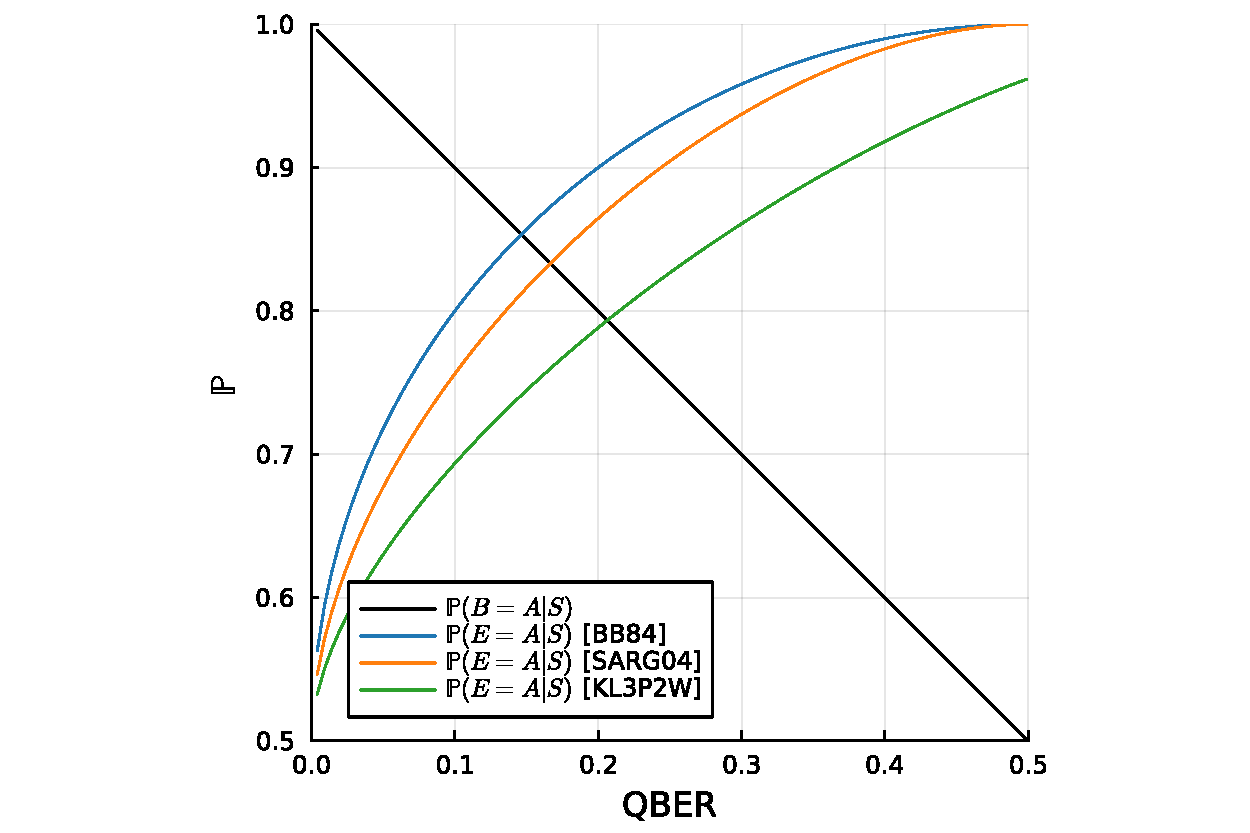
\includegraphics[width=1\linewidth]{figures/T.pdf}
    \caption{
        Comparison of the security of the protocols: BB84, SARG04, and KL3P2W
        counted with respect to QBER.
    }
    \label{fig:comp}
\end{figure}
\begin{figure}[hpt!]
    \centering
    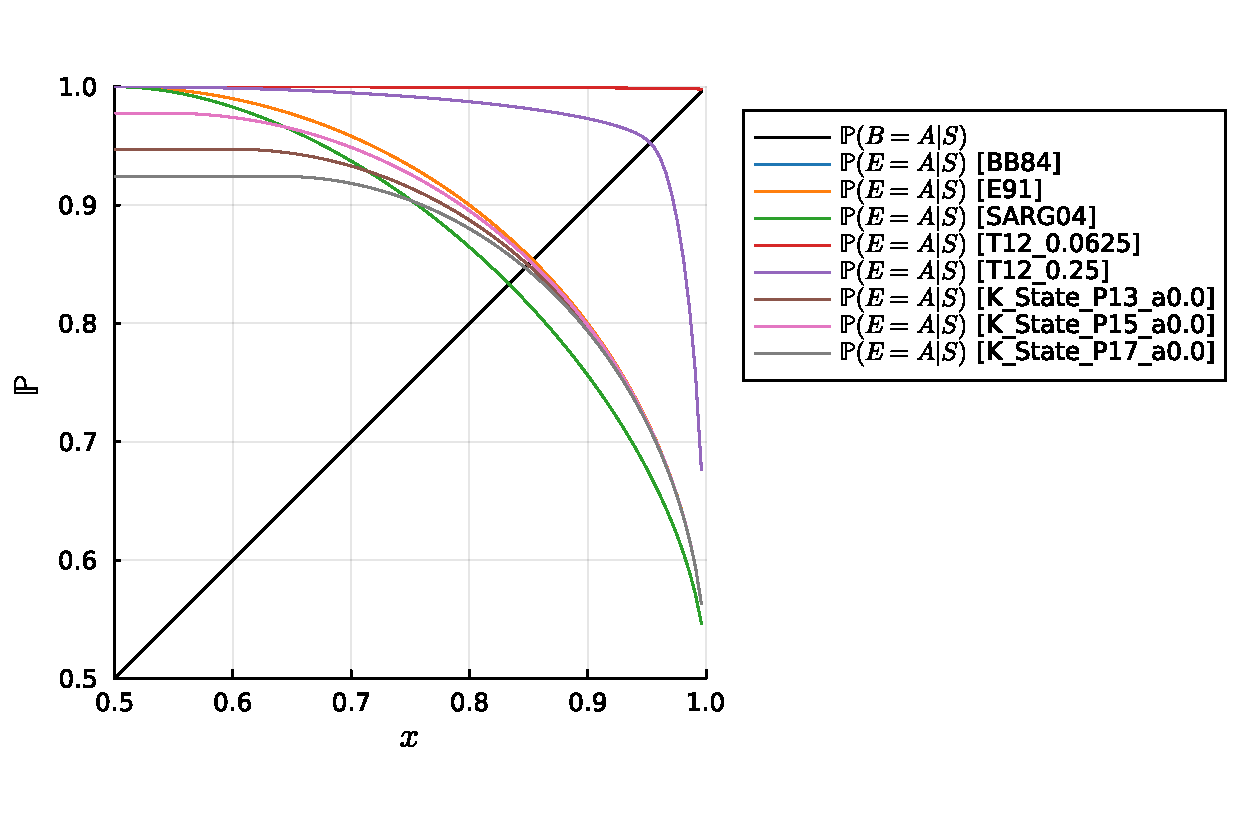
\includegraphics[width=1\linewidth]{figures/comparison.pdf}
    \caption{Comparison with various protocols}
    \label{fig:comp2}
\end{figure}


\section{Discussion}

Compared to existing QKD protocols, our scheme achieves a raw key rate of
approximately $10\%$, versus $25\%$ in BB84 \cite{BB84} and $\approx 22\%$ in
E91 \cite{ekert1991quantum}. This reduced rate reflects stricter acceptance
criteria but leads to stronger resilience against eavesdropping at higher QBER.

Although all QKD protocols ultimately rely on the no-cloning theorem, their
operational backbones differ. 
BB84 and B92 expose an eavesdropper through basis mismatch or imperfect state
discrimination, respectively. 
In contrast, entanglement-based protocols such as E91 exploit Bell inequality
violations and can offer device-independent security guaranties that go beyond
the no-cloning principle alone. 
Our protocol is based on explicit state discrimination, with non-uniform
preparation probabilities chosen to maximize the separation between Bob’s and
Eve’s success rates. The used state discrimination can be performed with and
without entanglement \cite{puchala2018strategies}, therefore, a proposed
protocol similar to B92 \cite{B92} can also have an entanglement version BBM92
\cite{B92ent}.

Our method, which relies on discrete registers and a deterministic decision
function $f$, is naturally restricted to DV-QKD. Extending the framework to
continuous-variable protocols remains an open direction. The T12 \cite{T12}
shown in Fig. \ref{fig:comp2} is treated as an unbalanced BB84 (the distribution
of probabilities is not uniform).
In our research, we do not consider threats that exist during practical
implementation like photon number splitting. 

The results (Table~\ref{fig:comp}) show that KL3P2W can limit Eve's information
gain more effectively than BB84 or the Six-State Protocol \cite{SSP} at elevated
QBER. This advantage comes from the explicit use of measurement discrimination
in both the choice of preparation probabilities and the acceptance rule. The
probabilities of sending the quantum state by Alice are not uniform and were
specifically chosen to ensure the best possible security.

By restricting Bob’s measurement to a SIC-POVM, the scheme gains mathematical
clarity. SIC-POVMs are informational complete, so Bob's outcome distribution
fully characterizes the input state, simplifying the analysis of Eve’s
actions.

The decision function $f(a,b)$ ensures that after postprocessing, the protocol
satisfies condition $P(A=B|S)=1$, that is, whenever the protocol accepts, the
keys match perfectly. Standard BB84 or six-state protocols rely on basis
reconciliation. Here, the reconciliation is built into the decision function
$f(a,b)$ and equivalence classes $R_a(a,b),R_b(a,b)$, making the structure more
flexible and adaptable.

Leaving Eve's strategy to be expressed as an operator $E$ (and eventually as a
binary measurement $\Upsilon_{f(a,b)}$), the scheme gives a flexible framework.
Eve is not tied to any particular intercept-resend strategy, but can in
principle use general quantum operations.

Using a black-box perspective, the protocol can be modified to achieve various
characteristics. For example, we can construct the protocol that $P(S) \to 1$
and $P(B=A|S) = 1$, which means the key ratio goes to $1$, but to guarantee the
security of our protocol, we need almost perfect QC. Moreover, in that case even
a small interaction with Eve will suspend the key generation $P_E(S) \to 0$.


\section{Methods} 

\subsection{Decision function}
Let $P = [P(b,a)]_{b,a}$ be a matrix of probabilities obtaining the label $a$
and $b$ for  Alice and Bob, respectively. Let us now assume that $P(b,a) > 0$
(noiseless, without the intervention of Eve). We analyze how $f$ looks like.
There are two possible scenarios:
\begin{enumerate}
    \item There are labels $a' \neq a$ and $b' \neq b$ such that $P' =
\begin{pmatrix} P_{b,a'} & P_{b,a} \\
    P_{b',a'} & P_{b',a} \end{pmatrix}= \begin{pmatrix} 0 & P_{b,a} \\
    P_{b',a'} & 0 \end{pmatrix}$. If the communication protocol $f$ agrees with
$P'$, that is, $a \in \{a,a'\}, b \in \{b,b'\}$, then $S$, Alice and Bob agree
that the key is $0$ for $a,b$ and $1$ for $a',b'$ or reversely, with probability
$50\%/50\%$. If $f$ does not find $P'$, then $\neg S$, the key generation is
aborted. In that case, $a',b'$ are unique.
    \item The case $(1)$ does not hold, and the protocol cannot generate a key
    (\(\neg S\)).
\end{enumerate}

\subsection{BB84 protocol as QKD-1q}
To determine the BB84 protocol in our framework (Fig. \ref{fig-protocol}) we
need the following parameters: 
\begin{itemize}
    \item Distribution: $P(a)$ for $a=1,\ldots,|R_a|$. 
    \item Quantum states: $ \ket{\psi_a}$ for $a=1,\ldots,|R_a|$ that are
    pairwise different.
    \item POVM: $\Omega = \{\proj{\phi_b}\}_b$ for $b=1,\ldots,|R_b|$ where the
effects are pairwise different.
    \item Decision function: $f(a, b)$.
\end{itemize} 

Originally, Alice creates a random bit, 0 or 1, and then randomly selects one of
her two bases $\{ \ket{0}, \ket{1}\}$ or $\{\ket{+}, \ket{-}\} $ and sends it to
Bob. As Bob does not know the basis the qubit were encoded in,  all he can do is
to select a basis at random to measure in the Z-basis or X-basis. 

For this purpose, Alice sends one of four quantum states $ \{ \ket{0}, \ket{1},
\ket{+}, \ket{-} \} $ with uniform distribution, e.g. $P(a) = \frac{1}{4} $ for
each $a$. Finally, Bob creates POVMs $\Omega$ with effects $\{
\frac{1}{2}\proj{0}, \frac{1}{2}\proj{1}, \frac{1}{2}\proj{+}, \frac{1}{2}
\proj{-} \} $. 
Then, the matrix of probabilities $P = [P(b,a)]_{b,a}$ is given by 
\begin{center}
\begin{tabular}{ |c|c|c|c| } 
 \hline
\cellcolor[HTML]{AA0044} 0 & \cellcolor[HTML]{AA0044} 1/8 & 1/16 & 1/16  \\
\hline  
 \cellcolor[HTML]{AA0044} 1/8 & \cellcolor[HTML]{AA0044} 0 & 1/16 & 1/16  \\
\hline 
 1/16 & 1/16 & \cellcolor[HTML]{AA0044} 0 & \cellcolor[HTML]{AA0044} 1/8  \\ 
\hline
 1/16 & 1/16 & \cellcolor[HTML]{AA0044} 1/8 & \cellcolor[HTML]{AA0044} 0 \\
\hline
\end{tabular}
\end{center}

In BB84, Alice and Bob jointly keep only the bits for which the bases were
consistent (they discard the rest).
So now we accept only the results marked in red (the upper left corner with
probability 1/2 and the lower right corner with probability 1/2). Then, the
function $f(a,b)$ is taken for pairs $(1,2)$ and $(3,4)$ with probability
$\frac{1}{2}$ for both pairs.

\begin{figure}[hpt!]
    \centering
    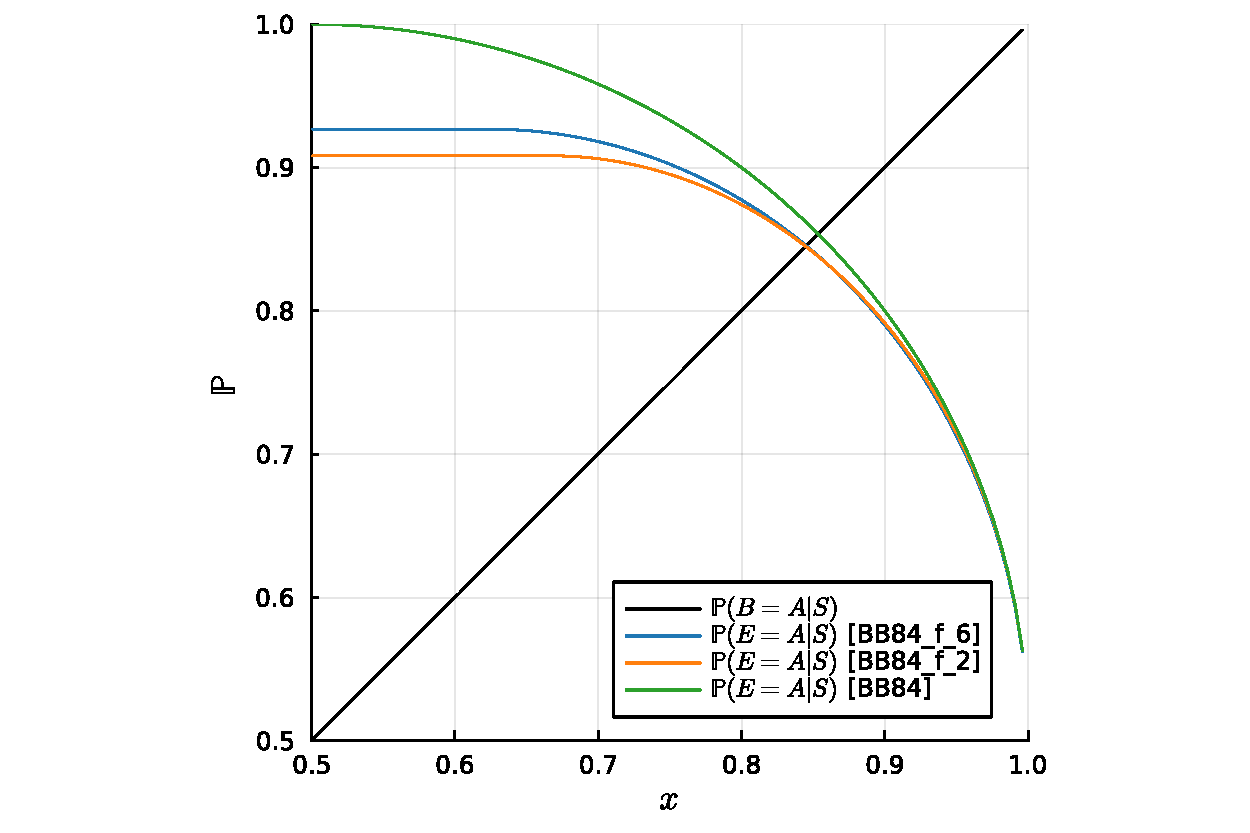
\includegraphics[width=1\linewidth]{figures/BB84_f.pdf}
    \caption{
        BB84 protocol with different decision functions. The origin decision
        function is described by green line. The modifications $f_2$ and
        $f_6$ are described by red and blue lines, respectively, obtaining
        the advantage over the origin one. Originally BB84 takes $P'$ given
        by indices $1,2$ and $3,4$. Modification $f_2$ takes indices $1,3$
        and $1,4$ while $f_6$ modification takes all index pairs $i,j$ for
        $i<j$.
    }
    \label{fig:enter-label}
\end{figure}

\subsection{Full procedure overview and Eve’s Attack Strategies}
Definition of Protocol Components:
\begin{enumerate}
    \item QKD-1q: $p_a$, $\ket{\psi_a}$, $\Omega$ and $f$.
    \begin{itemize}
    \item Distribution: $P(a)$ for $a=1,\ldots,L_a$. 
    \item Quantum states: $ \ket{\psi_a}$ for $a=1,\ldots,L_a$ that are pairwise
different.
    \item POVM: $\Omega = \{\proj{\phi_b}\}_b$ for $b=1,\ldots,L_b$ where
    effects are pairwise different. To generate $P(S) > 0$ and
    $P(A=B|S) = 1$ we need at least one $P'$. Let
    $2\le x\le \min(L_a,L_b)$ be a number such that
    $\mathrm{diag}([P_{b,a}]_{b,a=1}^x) = 0$, that means
    $\ket{\phi_b} \propto \ket{\psi^\perp_b}$ for $b=1,\ldots,x$.
    \item Decision function: $f(a, b)$ contains a list of $P'$ and a
    distribution to choose them $P(P')$.
    \item The action of observing Eve can be indexed by $P'$, that is,
$\Upsilon_{P'}$. If $S$ then $e \to E$. Otherwise, $e$ is discarded, but the
choice of $\Upsilon_{P'}$ does not change the statistics of $P_E(b,a)$.
\end{itemize}
    \item Acceptable ratio $x$, that is, $P_E(A=B|S) \ge x$. This component
    in the analysis ensures that DoS and mismatch attacks are limited.
    \item Error correction procedure (EC) that is defined based on $x$ and
$\min(\max P_E(E=A|S), \max P_E(E=B|S))$ a
    \item Privacy amplification method (PA) that is defined based on $x$,
    $\min(\max P_E(E=A|S), \max P_E(E=B|S))$ and EC.
\end{enumerate}
With such a created model, we reduce Eve's attacks to an optimization problem
over her best possible information gain, given that Alice and Bob enforce
$P(B=A|S)\ge x$ via EC and PA, these motivates the SDP, optimal Eve's strategy
must be consistent with these constraints.

Protocol:
\begin{enumerate}
    \item Making $X_1$ independent quantum experiments.
    \item $X_2$ of $X_1$ experiments have $S$.
    \item If $X_2 = 0$, then abort.
    \item Estimation of $P_E(A=B|S)$ based on part (log in size) of $X_2$.
    Alice has key $A_1 \ldots A_{X_3}$ and Bob $B_1 \ldots B_{X_3}$.
    \item If $P_E(A=B|S) < x$, then abort.
    \item Alice (or Bob, depending on the EC) samples a uniformly secret bit
    string of size $X_4$ and encodes it into a string $C$ of size $X_3$.
    She publicly announces a shifting sequence that takes her key
    $A_1 \ldots A_{X_3}$ and matches it with $C$. Bob does the same shift
    with his key.
    \item Alice and Bob use PA to define the secret key $K$ of size $X_5$.
\end{enumerate}

Eve attacks:
\begin{enumerate}
    \item Decreasing $P_E(S)$. If $P_E(S) = 0$, then attack succeeds.
    \item Decreasing $P_E(A=B|S)$. If $P_E(A=B|S) < x$, then attack succeeds.
    \item Increasing $P_E(A=E|S)$ if Alice generates secret or $P_E(B=E|S)$
    if Bob. If $P_E(E=A|S) \ge x$ (or $P_E(E=B|S) \ge x$), then attack
    succeeds.
\end{enumerate}

\subsection{QKD goal}
The goal of a QKD protocol is to ensure that Alice and Bob share a uniformly
random key of length $N$ such that $P(K_A=K_B)=1$ and $P(K_A=K_E)=0.5$ while Eve
has $0$ knowledge about it. The efficiency oof the procedure is evaluated
through the ratio:
\begin{equation}
    \begin{split}
        R(QKD, x) = P_E(S) \times \\
        \times \mathrm{Capacity}(P_E(B=A|S) \ge x) \times \\
        \times \mathrm{Extraction}(P_E(B=A|S), \\ 
        \min (\max P_E(E=A|S), \max P_E(E=B|S))),
    \end{split}
\end{equation}
which depends only on black-box measurements.

The optimization task is to find:
\begin{equation}
    x \to \arg \max_{QKD} R(QKD,x) 
\end{equation}

\subsection{Analysis of probabilities}
Independent probabilities: 
\begin{equation}
    P(a), P(P')
\end{equation}

Dependent probability:
\begin{equation}
    P(e,b|a,P')
\end{equation}

Probability of success:
\begin{equation}
    \begin{split}
P_E(S) &= \sum_{a,P'} P(a)P(P') P_E(S \mid a, P') \\
       &= \sum_{P'} P(P') \sum_{(a,b) \in P'} P(a) \sum_e P(e,b|a,P').
    \end{split}
\end{equation}


Probability of key compliance and success:
\begin{widetext}
\begin{equation}
    P_E(S \wedge K=A) = \sum_{P'} P(P') 
    \sum_{e,(a,b) \in P'} P(a) P_E(K=A,e,b|a,P').
\end{equation}
\end{widetext}

Probability of key compliance Bob and success:
\begin{widetext}
\begin{equation}
 P_E(S \wedge B=A) =\sum_{P'} P(P') \sum_{(a,b) \in P', a\neq b} P(a) \sum_e
P(e,b|a,P').
\end{equation}
\end{widetext}

Probability of key compliance Eve and success:
\small{
\begin{equation}
\begin{split}
    P_E(S \wedge E=A) &= \\ 
    &= \sum_{P'} P(P') \sum_{(a,b) \in P'} P(a) P(a',b|a,P').
\end{split}
\end{equation}}

\subsection{Semi Definite Programming}
We want to solve Eve's optimal guessing probability:
\begin{equation}
\begin{split}
   y(x) = \sup_E\left\{ P_E(E=A|S): P_E(B=A|S) \ge x\right\}.
\end{split}
\end{equation} 
Due to our QKD-1q construction, for any $E$, we have $P_E(S) \ge \epsilon > 0$
for some $\epsilon$.
Therefore,
\begin{equation}
y(x) = \max_E\left\{ P_E(E=A|S): P_E(B=A|S) \ge x\right\}
\end{equation}
is achievable. 
The defined Eve strategy:
\begin{equation}
E = \sum_{e,P'} \proj{e} \otimes \proj{P'} \otimes E_{e,P'} \ge 0
\end{equation}

The additional quantum network conditions: 
\begin{equation}
E = \sum_{e,P'} \proj{P'} \otimes E_{e,P'} = \Id_{P'} \otimes M
\end{equation}
and
\begin{equation}
\tr_{B}(M) = \Id_A
\end{equation}
But in the optimization problem $y(x)$ we can relax the last condition: $0 \neq
\tr_{B}(M) \propto \Id_A$ and the  problem reads:

\begin{widetext}
\begin{equation}
    \begin{split}
        y(x) &= \max_{\text{relaxed }E}\left\{ \frac{P_E(S \wedge E=A)}{P_E(S)}:
\frac{P_E(S \wedge B=A)}{P_E(S)} \ge x\right\}\\
        &= \max_{\text{relaxed }E}\left\{
        \frac{P_E(S \wedge E=A)}{P_E(S)}:
        \frac{P_E(S \wedge B=A)}{P_E(S)} \ge x, P_E(S)=1\right\}\\
        &= \max_{\text{relaxed }E}\left\{
        P_E(S \wedge E=A): P_E(S \wedge B=A) \ge x, P_E(S)=1\right\}.
    \end{split}
\end{equation}
\end{widetext}

The last formulation of $y(x)$ is SDP. From the optimal relaxed $E$ we get the
original and $P_E(S)$ by reassuring that $\tr_{B}(M) = \Id_A$.  \\

In conclusion, we need to compute:
\begin{equation}
    z(x) = \inf_{y \in \text{QKD-1q}} y(x).
\end{equation}

The problem can be summarized as a pseudocode: 
\begin{algorithm}[H]
\caption{SDP formulation of Eve’s optimal strategy}
\begin{algorithmic}[1]
\State \textbf{Variables:} Eve’s measurement operators $\{E_{e,P'}\} \succeq
0$
\State \textbf{Constraints:}
    \State \hspace{1em} $P_E(S) = 1$
    \State \hspace{1em} $P_E(S \wedge B=A) \ge x$
    \State \hspace{1em} $\tr_B(M) = \Id_A$  \Comment{Relax to $\tr_B(M) \propto
\Id_A$ if needed}
\State \textbf{Objective:} Maximize $P_E(S \wedge E=A)$
\end{algorithmic}
\end{algorithm}

\subsubsection{Optimal minimal case}
The calculated minimal case is equal to $L_a=2$ and $L_b=3$ with $x=2$, where
the optimal appears to be
\begin{itemize}
    \item $P(1)=P(2)=1/2$
    \item $\ket{\psi_1}=\ket{0},
\ket{\psi_2}=\sqrt{1-\epsilon}\ket{0}+\sqrt{\epsilon}\ket{1}$
    \item $\Omega = \{c\proj{\psi_1^\perp}, c\proj{\psi_2^\perp},
\rho_\epsilon\}$
\end{itemize}
for $\epsilon\to0$.

\subsection{Error correction and privacy amplification}

\subsection{Numerical artifact contract}
To bridge manuscript claims with reproducible computations, we define the output
interface expected from the codebase.
\begin{itemize}
    \item \texttt{three\_case\_curves.csv}: pointwise SKR curves with columns
    \texttt{case,epsilon,R,x\_opt,y\_opt}.
    \item \texttt{three\_case\_curves.pdf}/\texttt{three\_case\_curves.png}:
    publication figures generated from the CSV above.
    \item \texttt{validation\_points.csv}: validation grid with columns
    \texttt{epsilon,case1\_R,case2\_R,case3\_R,upper\_bound,gap\_case1,%
    gap\_case2,gap\_case3,best\_case,case1\_x\_opt,case2\_x\_opt,%
    case2\_y\_opt,case1\_best\_seed,case2\_best\_seed}.
    \item \texttt{validation\_summary.csv}: rows of type
    \texttt{stats}/\texttt{crossover} with columns
    \texttt{row\_type,case,epsilon,mean,std,min,max,best\_seed,best\_R,%
    crossover\_from,crossover\_to,crossover\_est\_eps,%
    bracket\_eps\_left,bracket\_eps\_right}.
    \item \texttt{validation\_meta.json}:
    machine-readable run metadata including
    \texttt{created\_at,eps\_min,eps\_max,eps\_step,eps\_count,restarts,%
    tol,seed,suppress\_warnings,git\_commit,runtime\_seconds}.
    \item \texttt{validation\_curves.pdf}/\texttt{validation\_curves.png} and
    \texttt{validation\_gaps.pdf}/\texttt{validation\_gaps.png}:
    manuscript-ready plots generated from \texttt{validation\_points.csv}.
    \item \texttt{n1\_points.csv}, \texttt{n1\_summary.csv},
    \texttt{n1\_meta.json}:
    Sprint 2A N=1 theorem-draft falsification artifacts generated on the
    $\epsilon$ grid with step $0.005$.
    \item \texttt{upper\_bound\_audit.csv}: row-wise verification that
    \texttt{upper\_bound} dominates \texttt{case1/case2/case3} over the same
    grid, with violation tolerance reported in \texttt{n1\_summary.csv}.
    \item \texttt{n1\_theorem\_curves.pdf}/\texttt{n1\_theorem\_curves.png}
    and
    \texttt{n1\_theorem\_mismatch.pdf}/\texttt{n1\_theorem\_mismatch.png}:
    manuscript-ready Sprint 2A plots generated from \texttt{n1\_points.csv}.
    \item \texttt{n1\_proof\_diagnostics.csv} and
    \texttt{n1\_proof\_diagnostics\_summary.csv}: Sprint 2B diagnostics for
    local optimality and SKR decomposition consistency in the positive-rate
    N=1 regime.
\end{itemize}
The accepted schema is the contract for subsequent automation of manuscript
tables and comparison figures.

\subsection{N=1 optimality theorem (draft)}
For the one-parameter family used in \texttt{case1}, we evaluate a draft
closed-form expression against independent numerical optimizers and a dense
scan baseline.
\begin{equation}
R_{N=1}^{\mathrm{draft}}(\epsilon) =
R_0\max\left(1-\frac{\epsilon}{\epsilon_c},0\right)^\alpha,
\end{equation}
with fixed constants
$R_0=0.893925772022$, $\epsilon_c=0.07$, and $\alpha=8$.

\paragraph{Theorem (draft, N=1).}
For $\epsilon \in [0,0.25]$, the draft candidate above is proposed as an
analytic surrogate for the restart-best numerical optimum in the N=1 family.
This statement is intentionally marked as a draft theorem and is supported by
explicit falsification diagnostics rather than a completed proof.

\paragraph{Proposition 1 (proved: parametric reduction).}
Within \texttt{case1}, protocol optimization reduces to a scalar search over
$x>0$ (equivalently $u=\log_{10}(x)$).
\textit{Proof sketch.}
The constructor \texttt{build\_case1\_protocol(x)} fixes
$p=(1,1)$, $q=(1)$, and states
$\ket{\psi_{1,0}}=(1,0)^T$, $\ket{\psi_{1,1}}=(1,x)^T$ up to normalization.
No additional free protocol parameters remain, so the outer family search is
one-dimensional.

\paragraph{Lemma 2 (KKT active-constraint criterion, draft).}
For fixed $x$ and $\epsilon$, define
\begin{equation}
    \begin{split}
        \PP_\epsilon(S,x)=\min_{J \succeq 0}\ &\mathrm{tr}(JQ_S)\\
        \mathrm{s.t.}\quad &\mathrm{Tr}_B(J)=I_2,\\
        &g_x(J):=
        \mathrm{tr}(JW_S)-x\,\mathrm{tr}(JQ_S)\ge 0.
    \end{split}
\end{equation}
Let $(J_x^\star,\lambda_x^\star,Y_x^\star,Z_x^\star)$ satisfy KKT conditions,
including
\begin{equation}
\lambda_x^\star g_x(J_x^\star)=0,\quad \lambda_x^\star \ge 0.
\end{equation}
Therefore, a proof that $\lambda_x^\star>0$ on the positive-rate region implies
that the Bob-agreement inequality is active:
$g_x(J_x^\star)=0$.

\paragraph{Remaining proof tasks.}
\begin{enumerate}
    \item \textbf{TODO-PROOF (Lemma 2 closure).} Prove $\lambda_x^\star>0$
    for positive-rate N=1 rows or state explicit counter-conditions.
    \item \textbf{Lemma 3 (TODO-PROOF: envelope regularity).} Establish the
    piecewise-smooth envelope conditions that motivate the
    $R_0,\epsilon_c,\alpha$ form.
    \item \textbf{Lemma 4 (TODO-PROOF: converse consistency).} Connect the
    fitted N=1 envelope to a rigorously stated upper-bound family and isolate
    the gap term.
\end{enumerate}

Sprint 2A evidence is summarized in
Table~\ref{tab:n1-theorem-summary} and
Figure~\ref{fig:n1-theorem-curves}. Full epsilon-grid rows are provided in
Table~\ref{tab:n1-theorem-grid-full-appendix}. Bound-audit diagnostics are
reported from \texttt{upper\_bound\_audit.csv}; for broad context on
capacity-style converse limits we refer to \cite{PirandolaAOP2020}.
Sprint 2B diagnostics are summarized in
Table~\ref{tab:n1-proof-diagnostics}. The decomposition mismatch is concentrated
at $\epsilon=0$, while local optimality checks pass on all positive-rate rows.
KKT dual multipliers are positive on all positive-rate rows, and active
sensitivity passes on 7/8 rows; the outlier is the boundary point
$\epsilon=0$ where $x_{\mathrm{active}}\approx 1$.
Lemma 2 is therefore supported on interior positive-rate points but remains
open at the boundary.

\begin{table}[ht]
\centering
\scriptsize
\caption{Sprint 2A N=1 theorem-draft evidence summary (rounded to 6 decimals).}
\label{tab:n1-theorem-summary}
\begin{tabular}{lc}
\hline
Metric & Value \\
\hline
max $|$numeric-scan$|$ & 0.000000 \\
mean $|$numeric-scan$|$ & 0.000000 \\
max $|$numeric-formula$|$ & 0.235688 \\
mean $|$numeric-formula$|$ & 0.007972 \\
target max $|$numeric-scan$| \le 0.000500$ & met \\
bound violations ($>10^{-7}$) & 0 \\
\hline
\end{tabular}
\end{table}

\begin{table}[ht]
\centering
\scriptsize
\caption{Sprint 2B proof diagnostics
(\texttt{local\_u\_step}=0.01, \texttt{x\_sensitivity\_step}=0.001).}
\label{tab:n1-proof-diagnostics}
\begin{tabular}{lc}
\hline
Metric & Value \\
\hline
positive-rate rows & 8 \\
local-optimality pass ratio & 1.000000 \\
active-sensitivity pass ratio & 0.875000 \\
active-sensitivity pass ratio, $\epsilon>0$ & 1.000000 \\
mean $(p_{\mathrm{plus}}-p_{\mathrm{active}})$ & 0.000963 \\
lambda-positive ratio & 1.000000 \\
max $|\lambda_{\mathrm{d}}-\lambda_{\mathrm{fd}}|$ all & 2087.580366 \\
max $|\lambda_{\mathrm{d}}-\lambda_{\mathrm{fd}}|$, $\epsilon>0$ & 0.010658 \\
first zero-rate epsilon & 0.040000 \\
$x$ monotone pre-zero & true \\
max decomposition abs. error & 0.065128 \\
max decomposition abs. error, $\epsilon>0$ & 0.000000 \\
mean decomposition abs. error & 0.008141 \\
\hline
\end{tabular}
\end{table}

\begin{figure}[ht]
\centering

\includegraphics[width=1\linewidth]
{../../results/sprint2_n1/n1_theorem_curves.pdf}
\caption{Sprint 2A N=1 theorem-draft curves: restart-best numeric, dense scan,
and draft formula.}
\label{fig:n1-theorem-curves}
\end{figure}

\subsection{Validation summary (production grid)}
We validated the numerical pipeline on $\epsilon \in [0, 0.25]$ with step
$0.01$, three restarts per $\epsilon$, tolerance $10^{-7}$, and deterministic
seeds. Table~\ref{tab:validation-case-summary} summarizes per-case maxima and
gap-to-bound behavior. Table~\ref{tab:validation-crossovers} reports winner
crossover estimates. Figure~\ref{fig:validation-curves} shows the production
validation curves.

\begin{table}[ht]
\centering
\scriptsize
\caption{Production-grid summary by protocol case.}
\label{tab:validation-case-summary}
\begin{tabular}{lccccc}
\hline
Case & Rmax & eps@Rmax & mean gap & mean std & max std \\
\hline
case1 & 0.893926 & 0.000000 & 0.403985 & 0.010433 & 0.271188 \\
case2 & 0.995895 & 0.000000 & 0.293813 & 0.000141 & 0.003664 \\
case3 & 0.333333 & 0.000000 & 0.298207 & 0.000000 & 0.000000 \\
\hline
\end{tabular}
\end{table}

\begin{table}[ht]
\centering
\scriptsize
\caption{Winner crossover estimates from production validation.}
\label{tab:validation-crossovers}
\begin{tabular}{ccccc}
\hline
from & to & est eps & left eps & right eps \\
\hline
case2 & case3 & 0.072514 & 0.070000 & 0.080000 \\
\hline
\end{tabular}
\end{table}

\begin{figure}[ht]
\centering

\includegraphics[width=1\linewidth]
{../../results/validation/validation_curves.pdf}
\caption{Production validation curves for case1, case2, case3, and upper bound.}
\label{fig:validation-curves}
\end{figure}

Full per-epsilon rows are listed in
Table~\ref{tab:validation-grid-full-appendix}. Canonical artifacts are tracked
under \texttt{results/validation}.

\section{Data availability}
The numerical datasets used for curve generation are produced directly by the
analysis scripts and stored as CSV/JSON artifacts in the project repository.
\section{Code availability}
Code and reproducibility artifacts are maintained in the project repository.
\textbf{TODO(repository URL):} replace this sentence with the final persistent
public URL before submission.

\appendix
\section{Protocol Landscape Catalog}
This appendix consolidates the protocol-by-protocol notes used to position the
proposed QKD-1q framework.

\subsection{Prepare-and-measure family}
\begin{itemize}
    \item \textbf{BB84} is the baseline four-state prepare-and-measure
    protocol with basis sifting \cite{BB84}.
    \item \textbf{B92} uses two non-orthogonal states and shifts complexity
    into Bob's discrimination step \cite{B92}.
    \item \textbf{Six-state (SSP)} extends BB84 by adding a third mutually
    unbiased basis \cite{SSP}.
    \item \textbf{SARG04} modifies reconciliation/post-selection to improve
    robustness against multi-photon attacks in weak-coherent implementations
    \cite{SARG04}.
    \item \textbf{T12} uses asymmetric basis probabilities and decoy-style
    operation to improve practical key throughput \cite{T12}.
    \item \textbf{DPS-QKD} encodes information in phase differences of
    sequential pulses and targets high-rate optical links \cite{DPS2002}.
\end{itemize}

\subsection{Entanglement-based and DI-related family}
\begin{itemize}
    \item \textbf{E91} uses Bell-correlation checks to monitor eavesdropping
    and certify security structure \cite{ekert1991quantum}.
    \item \textbf{BBM92} provides an entanglement-based counterpart to
    BB84-style key extraction \cite{B92ent}.
    \item \textbf{DI-QKD} advances toward security claims that rely less on
    trusted implementation internals and more on observed nonlocal statistics
    \cite{DIQKDReview2023}.
\end{itemize}

\subsection{MDI and long-distance-oriented family}
\begin{itemize}
    \item \textbf{MDI-QKD} removes trust in measurement devices by relocating
    detection to an untrusted relay \cite{LoCurtyQi2012}.
    \item \textbf{Twin-field QKD} improves repeaterless rate-distance behavior
    and has become a key long-distance reference point \cite{rate_distance}.
\end{itemize}

\subsection{Position of the present protocol}
The protocol in this manuscript remains in the prepare-and-measure class and
keeps single-qubit transmission as the primitive. Its distinguishing axis is
optimization of post-selection and state/measurement geometry to maximize
Bob--Eve discrimination gap under a fixed channel-noise model.

\subsection{Full production validation grid}
\begin{table*}[t]
\centering
\scriptsize
\caption{Full epsilon-grid validation rows from
\texttt{results/validation/validation\_points.csv}.}
\label{tab:validation-grid-full-appendix}
\begin{tabular}{cccccc}
\hline
$\epsilon$ & case1\_R & case2\_R & case3\_R & upper\_bound & best\_case \\
\hline
0.000000 & 0.893926 & 0.995895 & 0.333333 & 1.000000 & case2 \\
0.010000 & 0.151535 & 0.460156 & 0.310512 & 0.931537 & case2 \\
0.020000 & 0.060367 & 0.400621 & 0.291880 & 0.875639 & case2 \\
0.030000 & 0.020629 & 0.359967 & 0.274776 & 0.824327 & case2 \\
0.040000 & 0.000000 & 0.321941 & 0.258651 & 0.775954 & case2 \\
0.050000 & 0.000000 & 0.285919 & 0.243249 & 0.729748 & case2 \\
0.060000 & 0.000000 & 0.251535 & 0.228421 & 0.685262 & case2 \\
0.070000 & 0.000000 & 0.218547 & 0.214068 & 0.642204 & case2 \\
0.080000 & 0.000000 & 0.186786 & 0.200123 & 0.600368 & case3 \\
0.090000 & 0.000000 & 0.156124 & 0.186534 & 0.559602 & case3 \\
0.100000 & 0.000000 & 0.126466 & 0.173264 & 0.519792 & case3 \\
0.110000 & 0.000000 & 0.097736 & 0.160281 & 0.480844 & case3 \\
0.120000 & 0.000000 & 0.069871 & 0.147562 & 0.442685 & case3 \\
0.130000 & 0.000000 & 0.042821 & 0.135085 & 0.405254 & case3 \\
0.140000 & 0.000000 & 0.016545 & 0.122833 & 0.368500 & case3 \\
0.150000 & 0.000000 & 0.000000 & 0.110793 & 0.332380 & case3 \\
0.160000 & 0.000000 & 0.000000 & 0.098953 & 0.296858 & case3 \\
0.170000 & 0.000000 & 0.000000 & 0.087301 & 0.261903 & case3 \\
0.180000 & 0.000000 & 0.000000 & 0.075829 & 0.227486 & case3 \\
0.190000 & 0.000000 & 0.000000 & 0.064529 & 0.193586 & case3 \\
0.200000 & 0.000000 & 0.000000 & 0.053393 & 0.160179 & case3 \\
0.210000 & 0.000000 & 0.000000 & 0.042416 & 0.127249 & case3 \\
0.220000 & 0.000000 & 0.000000 & 0.031593 & 0.094780 & case3 \\
0.230000 & 0.000000 & 0.000000 & 0.020919 & 0.062757 & case3 \\
0.240000 & 0.000000 & 0.000000 & 0.010389 & 0.031167 & case3 \\
0.250000 & 0.000000 & 0.000000 & 0.000000 & 0.000000 & case3 \\
\hline
\end{tabular}
\end{table*}

\subsection{Full N=1 theorem-draft mismatch grid}
\begin{table*}[p]
\centering
\scriptsize
\caption{Full Sprint 2A N=1 mismatch rows from
\texttt{results/sprint2\_n1/n1\_points.csv}.}
\label{tab:n1-theorem-grid-full-appendix}
\begin{tabular}{cccccc}
\hline
$\epsilon$ & numeric\_R & scan\_R & formula\_R & $|$n-s$|$ & $|$n-f$|$ \\
\hline
0.000000 & 0.896954 & 0.896954 & 0.893926 & 0.000000 & 0.003028 \\
0.005000 & 0.258422 & 0.258422 & 0.494110 & 0.000000 & 0.235688 \\
0.010000 & 0.153844 & 0.153844 & 0.260452 & 0.000000 & 0.106608 \\
0.015000 & 0.096190 & 0.096190 & 0.129843 & 0.000000 & 0.033653 \\
0.020000 & 0.060359 & 0.060359 & 0.060573 & 0.000000 & 0.000214 \\
0.025000 & 0.036952 & 0.036952 & 0.026075 & 0.000000 & 0.010877 \\
0.030000 & 0.020692 & 0.020692 & 0.010162 & 0.000000 & 0.010530 \\
0.035000 & 0.008187 & 0.008187 & 0.003492 & 0.000000 & 0.004695 \\
0.040000 & 0.000000 & 0.000000 & 0.001017 & 0.000000 & 0.001017 \\
0.045000 & 0.000000 & 0.000000 & 0.000237 & 0.000000 & 0.000237 \\
0.050000 & 0.000000 & 0.000000 & 0.000040 & 0.000000 & 0.000040 \\
0.055000 & 0.000000 & 0.000000 & 0.000004 & 0.000000 & 0.000004 \\
0.060000 & 0.000000 & 0.000000 & 0.000000 & 0.000000 & 0.000000 \\
0.065000 & 0.000000 & 0.000000 & 0.000000 & 0.000000 & 0.000000 \\
0.070000 & 0.000000 & 0.000000 & 0.000000 & 0.000000 & 0.000000 \\
0.075000 & 0.000000 & 0.000000 & 0.000000 & 0.000000 & 0.000000 \\
0.080000 & 0.000000 & 0.000000 & 0.000000 & 0.000000 & 0.000000 \\
0.085000 & 0.000000 & 0.000000 & 0.000000 & 0.000000 & 0.000000 \\
0.090000 & 0.000000 & 0.000000 & 0.000000 & 0.000000 & 0.000000 \\
0.095000 & 0.000000 & 0.000000 & 0.000000 & 0.000000 & 0.000000 \\
0.100000 & 0.000000 & 0.000000 & 0.000000 & 0.000000 & 0.000000 \\
0.105000 & 0.000000 & 0.000000 & 0.000000 & 0.000000 & 0.000000 \\
0.110000 & 0.000000 & 0.000000 & 0.000000 & 0.000000 & 0.000000 \\
0.115000 & 0.000000 & 0.000000 & 0.000000 & 0.000000 & 0.000000 \\
0.120000 & 0.000000 & 0.000000 & 0.000000 & 0.000000 & 0.000000 \\
0.125000 & 0.000000 & 0.000000 & 0.000000 & 0.000000 & 0.000000 \\
0.130000 & 0.000000 & 0.000000 & 0.000000 & 0.000000 & 0.000000 \\
0.135000 & 0.000000 & 0.000000 & 0.000000 & 0.000000 & 0.000000 \\
0.140000 & 0.000000 & 0.000000 & 0.000000 & 0.000000 & 0.000000 \\
0.145000 & 0.000000 & 0.000000 & 0.000000 & 0.000000 & 0.000000 \\
0.150000 & 0.000000 & 0.000000 & 0.000000 & 0.000000 & 0.000000 \\
0.155000 & 0.000000 & 0.000000 & 0.000000 & 0.000000 & 0.000000 \\
0.160000 & 0.000000 & 0.000000 & 0.000000 & 0.000000 & 0.000000 \\
0.165000 & 0.000000 & 0.000000 & 0.000000 & 0.000000 & 0.000000 \\
0.170000 & 0.000000 & 0.000000 & 0.000000 & 0.000000 & 0.000000 \\
0.175000 & 0.000000 & 0.000000 & 0.000000 & 0.000000 & 0.000000 \\
0.180000 & 0.000000 & 0.000000 & 0.000000 & 0.000000 & 0.000000 \\
0.185000 & 0.000000 & 0.000000 & 0.000000 & 0.000000 & 0.000000 \\
0.190000 & 0.000000 & 0.000000 & 0.000000 & 0.000000 & 0.000000 \\
0.195000 & 0.000000 & 0.000000 & 0.000000 & 0.000000 & 0.000000 \\
0.200000 & 0.000000 & 0.000000 & 0.000000 & 0.000000 & 0.000000 \\
0.205000 & 0.000000 & 0.000000 & 0.000000 & 0.000000 & 0.000000 \\
0.210000 & 0.000000 & 0.000000 & 0.000000 & 0.000000 & 0.000000 \\
0.215000 & 0.000000 & 0.000000 & 0.000000 & 0.000000 & 0.000000 \\
0.220000 & 0.000000 & 0.000000 & 0.000000 & 0.000000 & 0.000000 \\
0.225000 & 0.000000 & 0.000000 & 0.000000 & 0.000000 & 0.000000 \\
0.230000 & 0.000000 & 0.000000 & 0.000000 & 0.000000 & 0.000000 \\
0.235000 & 0.000000 & 0.000000 & 0.000000 & 0.000000 & 0.000000 \\
0.240000 & 0.000000 & 0.000000 & 0.000000 & 0.000000 & 0.000000 \\
0.245000 & 0.000000 & 0.000000 & 0.000000 & 0.000000 & 0.000000 \\
0.250000 & 0.000000 & 0.000000 & 0.000000 & 0.000000 & 0.000000 \\
\hline
\end{tabular}
\end{table*}

\clearpage
\bibliographystyle{ieeetr}
\bibliography{qkd}

\section*{Acknowledgements}
  PL is supported by the Ministry of Education, Youth and Sports of the Czech
Republic through the e-INFRA CZ (ID:90254), with the financial support of the
European Union under the REFRESH – Research Excellence For
REgionSustainability and
High-tech Industries project number CZ.10.03.01/00/22\_003/0000048 via the
Operational Programme Just Transition.  
RK is supported by the European Union under the REFRESH – Research Excellence
For REgionSustainability and
High-tech Industries project number CZ.10.03.01/00/22\_003/0000048 via the
Operational Programme Just Transition.  
\section*{Author Contributions}
R.K. developed the theoretical framework and primary manuscript draft. P.L.
implemented and curated the computational experiments and generated the figures.
\textbf{TODO(author list):} add final contribution statements for any additional
co-authors before submission.
\section*{Competing interests}
The authors declare no conflict of interest.
\end{document}
